\documentclass[a4paper,twoside,ngerman]{scrreprt}


%
% Packages
%

\usepackage[pdftex]{graphicx}
\usepackage{pdfpages}
\usepackage{a4}
\usepackage[ngerman, english]{babel}
\usepackage[utf8]{inputenc}
\usepackage{bibgerm}
%\usepackage[colorlinks=true,linkcolor=blue]{hyperref}
\usepackage{xcolor}

\usepackage{cite}
\usepackage{url}
\usepackage{svn}
\usepackage{listings}
\usepackage{helvet}
\usepackage[bf]{caption}
\usepackage{color}
\usepackage{epsfig}
\usepackage{enumerate}
\usepackage[acronym]{glossaries} 
\usepackage{array}

\makeglossaries

\newglossaryentry{sample}{name={sample},
description={a sample entry}}

\newacronym[\glsshortpluralkey=cas,\glslongpluralkey=contrived
acronyms]{aca}{aca}{a contrived acronym}

%
% Custom Commands
%
\newcommand{\HRule}{\rule{\linewidth}{0.5mm}}
%unused
\newcommand\etc{\textsl{etc}}
\newcommand\eg{\textsl{eg.}\ }
\newcommand\etal{\textsl{et al.}}
\newcommand\Quote[1]{\lq\textsl{#1}\rq}
\newcommand\fr[2]{{\textstyle\frac{#1}{#2}}}
\newcommand\miktex{\textsl{MikTeX}}
\newcommand\comp{\textsl{The Companion}}
\newcommand\nss{\textsl{Not so Short}}

%
% Document
%
\begin{document}
	% Titelseite
	%-----------------------------------------------------------
\begin{titlepage}
 
\begin{center}
 
 
% Upper part of the page

\includegraphics[width=0.15\textwidth]{./img/logo}\\[2cm]
 

 
\textsc{\Large Bachelor Arbeit}\\[0.5cm]
 
 
% Title
\HRule \\[0.4cm]
{ \huge \bfseries Handschrifterkennung mit Android}\\[0.4cm]
 
\HRule \\[1.5cm]
 
% Author and supervisor
\begin{minipage}{0.4\textwidth}
\begin{flushleft} \large
\emph{Autoren:}\\
Julian \textsc{Hanhart}\\
Dominik \textsc{Giger}
\end{flushleft}
\end{minipage}
\begin{minipage}{0.4\textwidth}
\begin{flushright} \large
\emph{Betreuer:} \\ 
Dipl. El.-Ing. ETH / BWI Alexander \textsc{Bosshard}\\
 
\end{flushright}
\end{minipage}
 
\vfill
 
% Bottom of the page
\textsc{Winterthur}\\
{\large \today}
 
\end{center}
 
\end{titlepage}
%-----------------------------------------------------------

	\newpage
	\thispagestyle{empty}
	\mbox{}

	% Abstract / Management Summary (ev. Abstract on Title-Page)
	\selectlanguage{ngerman}

\begin{abstract}
\chapter*{Zusammenfassung}
\thispagestyle{empty}
\selectlanguage{ngerman}

\begin{abstract}
\chapter*{Zusammenfassung}
\thispagestyle{empty}
\selectlanguage{ngerman}

\begin{abstract}
\chapter*{Zusammenfassung}
\thispagestyle{empty}
\input{../abstract/abstract.txt}
\end{abstract}

\begin{otherlanguage}{english}
\begin{abstract}
\chapter*{Abstract}
\thispagestyle{empty}
\input{../abstract/abstract_en.txt}
\end{abstract}
\end{otherlanguage}
\end{abstract}

\begin{otherlanguage}{english}
\begin{abstract}
\chapter*{Abstract}
\thispagestyle{empty}
\input{../abstract/abstract_en.txt}
\end{abstract}
\end{otherlanguage}
\end{abstract}

\begin{otherlanguage}{english}
\begin{abstract}
\chapter*{Abstract}
\thispagestyle{empty}
\input{../abstract/abstract_en.txt}
\end{abstract}
\end{otherlanguage}

	
	\newpage
	\thispagestyle{empty}
	\mbox{}
	
	% BA Erklärung
	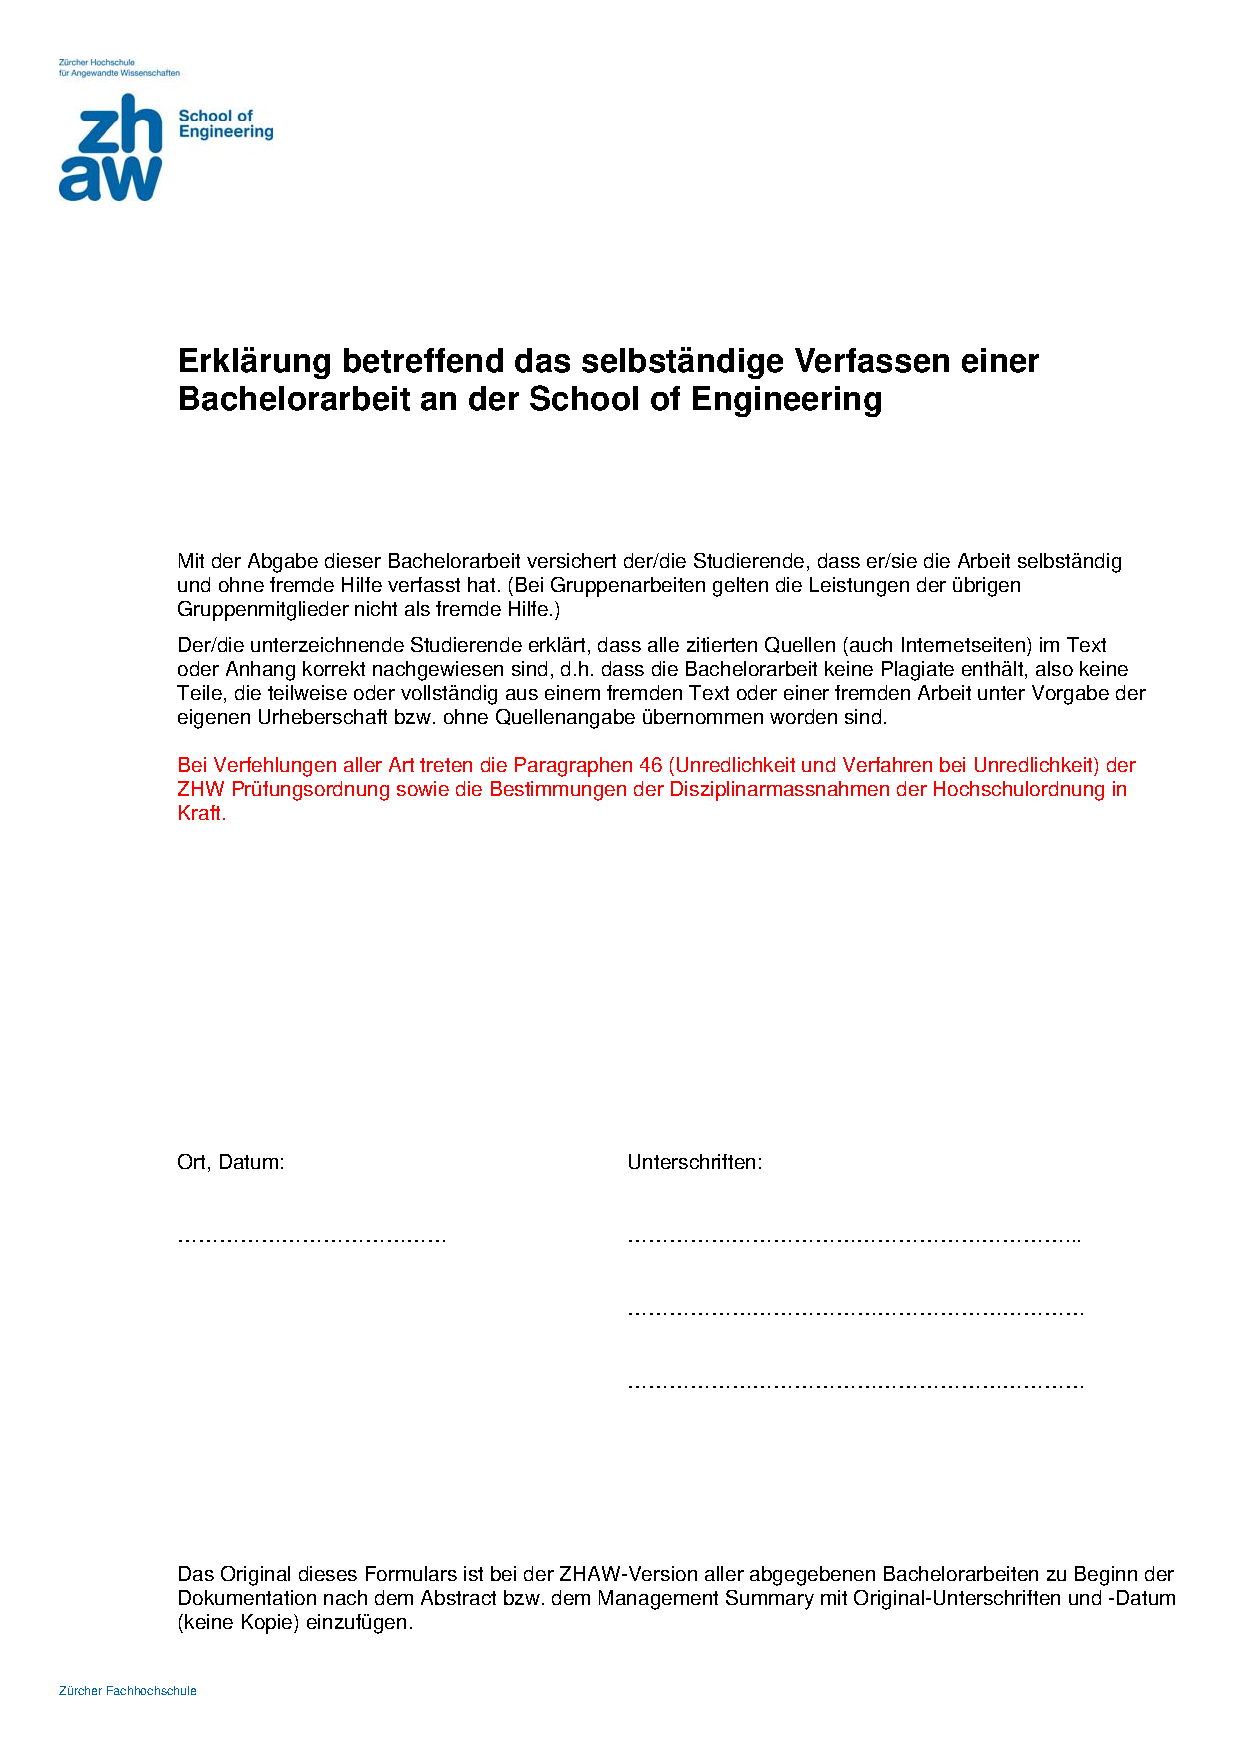
\includepdf[pagecommand={\thispagestyle{empty}},scale=1.0]{inc/Erklaerung_BA.pdf}
	
	\newpage
	\thispagestyle{empty}
	\mbox{}

	% Römische Seitenzahlen
	\newpage
	\renewcommand{\thepage}{\Roman{page}}
	\setcounter{page}{1}
	
	% Content
	\tableofcontents

	% Verzeichnisse
	% Abbildungen
	\listoffigures
	% Tabellen
	\listoftables
	% Listings
	\definecolor{listingbg}{HTML}{99CCCC}
	\renewcommand{\ttdefault}{pcr}
	\lstset{keywordstyle=\bfseries,basicstyle=\ttfamily}
	\lstset{language=Java, backgroundcolor=\color{listingbg}, frame=single, framerule=1pt,
		firstnumber=auto, numbers=left, numberstyle=\tiny, stepnumber=1, numbersep=8pt, 
		captionpos=b, tabsize=2, inputencoding=latin1, showstringspaces=false,
		aboveskip=0.6cm}
	\lstlistoflistings
	
	% Begin Inhalt
	% Seitenzahl auf Arabisch wechseln
	\newpage
	\renewcommand{\thepage}{\arabic{page}}
	\setcounter{page}{1}
	

	\part{Einleitung}
		\chapter{Aufgabenstellung}
Die Studenten realisieren eine Software in Android für das Erkennen von Handschrift, welche via Touchscreen eingegeben wird.

*Die Studierenden entwerfen eine Software, welche Touchscreen-Eingaben erkennt und auf dem Bildschirm wiedergibt
*Die Software soll sowohl einzelne Zeichen als auch mehrere zusammenhängende Zeichen („Schnürlischrift“) erkennen.
*Wenn der Finger angehoben wird, bedeutet das das Ende des Schriftzugs
*Die Erkennung verfolgt den Ansatz, dass verschiedene Zeichen sich aus Mikrogesten zusammensetzen. Diese Mikrogesten kommen in mehreren Zeichen vor.
*Die Applikation wird derart realisiert, dass die übrigen Funktionen des Mobilgerätes nicht behindert werden. Sie verfügt über die nötigen Bedienelemente (z.B. Bildschirm löschen etc.)

		\chapter{Resultate}
% - bessere Algorithmen zur MG-Erkennung
% - Character-Erkennung mit Graph
% - zwei MG-Varianten mit passenden Graphen
% - Import, Export, Visualisierung Graph
% - Software zum testen der Mikrogesten-Erkennung
% - Ersatz für das Keyboard im Android Betriebssystem
% - ???
% - Profit.

\begin{enumerate}
\item \textbf{Entwicklung einer Input-Method und Handschrifterkennungs-Service für Android} \\ 
Die erstellte Input-Method kann als Ersatz für das Standard-Keyboard von Android verwendet werden. Für die Erkennung der Buchstaben greift sie auf den Service zu, der die gesamte Erkennungs-Logik enthält und von der Input-Method unabhängig läuft.
Der Service ist komplett modular aufgebaut, was es erlaubt auf sehr einfache Weise die Logik zur Buchstabenerkennung zu ändern.

\item \textbf{Zwei Varianten für die Aufteilung von Pfaden in Mikrogesten} \\
Wir haben zwei verschiedene Varianten von Mikrogesten implementiert und verglichen. 

\item \textbf{Buchstaben-Erkennung basierend auf einem Graphen} \\
Für jede der Mikrogesten-Varianten haben wir einen Graph erstellt, welcher mit Hilfe der erkannten Mikrogesten einen Buchstaben auswählt. Für den Graph haben wir ausserdem noch Import-, Export- und automatische Visualisierungs-Funktionalitäten umgesetzt.

\item \textbf{Neue und verbesserte Algorithmen für die Mikrogesten-Erkennung} \\
Wir haben einen neuen Ansatz entwickelt, um Mikrogesten zu erkennen. Statt in einem Schritt alle verschiedenen Mikrogesten zu erkennen und bestimmen, wird der Pfad über mehrere Stufen verarbeitet. 

\end{enumerate}


		\chapter{Aufbau Report}
Der Report ist im Prinzip in drei Teile aufgeteilt:
\begin{itemize}
\item Theoretischer Hintergrund
\item Lösung / Umsetzung
\item Diskussion
\end{itemize}

Der Theoretische Hintergrund beschreibt dabei die Idee, wie die Handschrift erkannt werden soll. 

Die Lösung zeigt die Umsetzung der theoretischen Ideen in einem Java Programm. In diesem Teil werden vor allem die Algorithmen vorgestellt, die wir verwenden.

Die Diskussion enthält den Vergleich der verschiedenen Ansätzen. Ausserdem werden dort noch einige Vorschläge gemacht, wie man die von uns erstellte Lösung noch verbessern kann.		

		\chapter{Vorgehensweise}
Für die Lösung des Problems gibt es schon einen Ansatz aus einer vorhergehenden Arbeit. Wir werden den vorgeschlagenen Ansaz aus dieser Arbeit in einem Prototypen umsetzen. Dieser Prototyp wird jedoch so aufgebaut, dass jeder Teil der Erkennung beliebig ausgetauscht werden kann. Damit können wir nicht nur eine Variante, sondern für jeden Schritt mehrere testen. Nach dem Vergleich der verschiedenen Varianten werden wir die besten auswählen und damit die Release-Version für Android erstellen.

Im Endeffekt werden wir zwei verschiedene Erkennungsvarianten testen: Variante A ist aus der vorhergehenden Arbeit übernommen und Variante B wird durch uns selbst erstellt. Der Vergleich basiert schlussendlich auf der Erkennungsrate für eine bestimmte Anzahl zufällig ausgewählter Zeichen.

	\part{Theoretischer Hintergrund}
		\chapter{Mikrogesten}

Die grundsätzliche Idee zur Handschrifterkennung ist die Unterteilung der Schrift in sogenannte Mikrogesten. Eine Mikrogeste ist eine simple Bewegung, die beim Schreiben ausgeführt wird. Jeder Buchstabe soll dann aus solchen Mikrogesten aufgebaut werden können. 
Es ist nun natürlich möglich diese Mikrogesten auf beliebige Art zu definieren. Die Hauptkriterien sind, dass die Gesten so einfach wie möglich sein sollen (Für eine optimale Erkennung) und sich untereinander möglichst stark unterscheiden. Je weniger solche Gesten man braucht, desto besser. Man kann jedoch nicht beliebig grobe Gesten wählen, da immer noch alle möglichen Zeichen einzigartig aus solchen Gesten zusammen gebaut werden müssen.

\begin{figure}[h!]
  \centering
    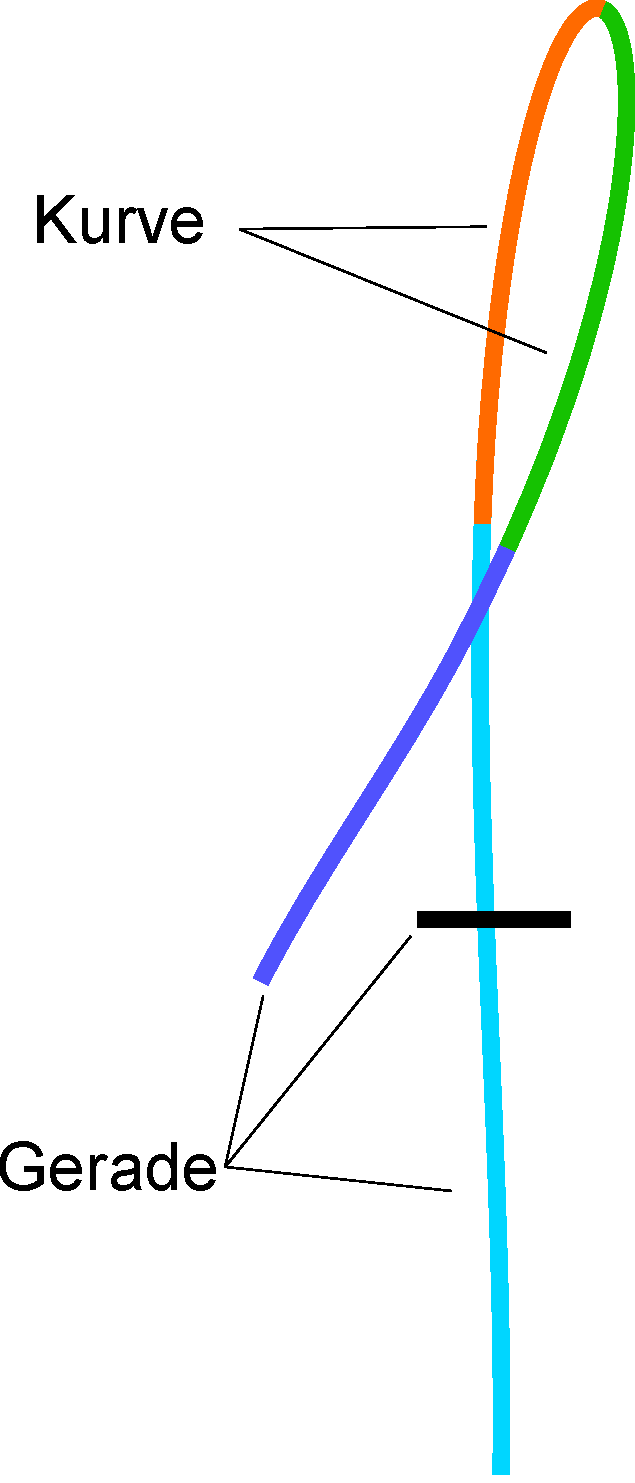
\includegraphics[width=0.2\textwidth]{./img/mikrogesten_beispiel.pdf}
  \caption{Beispiel für die Auftrennung des Buchstaben 'f' in Mikrogesten.}
  \label{mikrogeste_beispiel}
\end{figure}

In der Abbildung \ref{mikrogeste_beispiel} sieht man eine mögliche Aufteilung des Buchstaben 'f' in die Mikrogesten \emph{Kurve} und \emph{Gerade}. Der Buchstabe wird also durch die Abfolge Gerade-Kurve-Kurve-Gerade-Gerade definiert. Nur zwei Mikrogesten sind allerdings zu wenige um alle Zeichen eindeutig abzubilden.

\section{Eigenschaften}
Die Mikrogesten müssen genau definiert werden und können mehr als eine Eigenschaft besitzen:

\subsubsection{Form}
Es ist naheliegend die Mikrogesten hauptsächlich anhand ihrer Form zu unterscheiden. Diese Eigenschaft reicht jedoch nicht, um alle Buchstaben einzigartig zu beschreiben. Zum Beispiel könnte ein 'b' und ein 'p' beides als Gerade-Kreis beschrieben werden. 

\subsubsection{Ausrichtung}
Die Ausrichtung kann auch eine wichtige Eigenschaft sein, z.B. um Querstriche von Längsstrichen zu unterscheiden. Es bietet sich an, die Mikrogesten in eine diskrete Anzahl Richtungen abzubilden, um später die Erkennung im Graph zu vereinfachen.

\subsubsection{Länge}
Für Geraden kann die Länge eine wichtige Rolle spielen: Zum Beispiel ist der Unterschied zwischen 'q' und 'a' nur die Länge der Geraden.  Die Länge wird normalerweise nach dem Liniensystem der Schrift definiert (siehe Abbildung \ref{liniensystem}). Es wird unterschieden zwischen Linien die nur Mittellänge haben und solchen die Ober- oder Unterlänge haben.

\subsubsection{Position}
Die Schrift kann in drei Bereiche Unterteilt werden: Mittel-, Unter- und Oberlänge \cite{typo_linien}. Die Mikrogesten können sich generell in einem oder zwei dieser Bereiche befinden. Dies kann in spezialfällen die Unterscheidung ermöglichen: Zum Beispiel Besitzen 'p' und 'b' den gleichen Aufbau, jedoch befindet sich die Gerade an einer anderen Position.

\begin{figure}[h!]
  \centering
    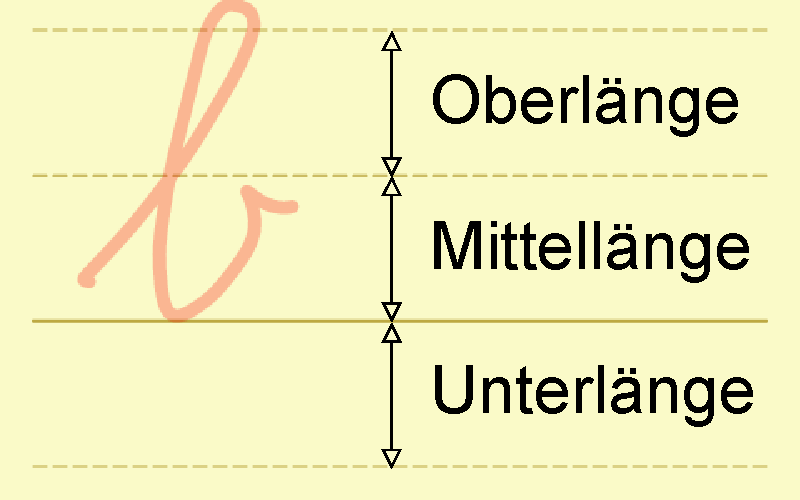
\includegraphics[width=0.4\textwidth]{./img/liniensystem.pdf}
  \caption{Unterteilung der Buchstaben in Mittel-, Unter- und Oberlänge}
  \label{liniensystem}
\end{figure}

\section{Typen}
\subsection{Variante A}
Variante A der Mikrogesten haben wir aus der bestehenden Projektarbeit \cite{zeichenerkennung_pa} zu diesem Thema übernommen: 

Es sind folgende Mikrogesten definiert:
\begin{itemize}
\item Gerade
\item Spitzkehre
\item Schwache Krümmung
\item Starke Krümmung
\end{itemize}

Es wird ausserdem noch berücksichtigt, ob der erkannte Buchstabe Ober- oder Unterlänge hat, um ähnliche Buchstaben zu unterscheiden. Richtung und Position der Mikrogesten werden nicht berücksichtigt.

\subsection{Variante B}
Variante B wurde von uns selbst erarbeitet, um eine bessere Toleranz gegenüber unterschiedlichen Schreibstilen zu erhalten:\begin{itemize}
\item Kreis
\item Halbkreis
\item Lange Gerade
\item Kurze Gerade
\end{itemize}

Die Bezeichnungen Kreis und Halbkreis könnten etwas irreführend sein: Die Pfade müssen nicht genau kreisförmig sein, sondern jeder geschlossene Pfad gilt als Kreis und jeder gebogene Pfad gilt als Halbkreis. Es wird zusätzlich noch die Position und Richtung der Mikrogesten berücksichtigt. Die daraus resultierenden Kombinationen sind in Tabelle \ref{varb_directions} ersichtlich.

\begin{table}[h!]
  \begin{center}
\[
    \begin{array}{l | c | c }
    Richtung & Halbkreis & Gerade \\
    \hline
   \mbox{Vertikal} & \subset & | \\
    \mbox{Vorwärts} & \cap & \backslash \\
    \mbox{Horizontal} & \supset & - \\
    \mbox{Rückwärts} & \cup & / \\
    \hline
    \end{array}
\]
  \end{center}
  \caption{Die vier Richtungen für Halbkreis und Gerade}
  \label{varb_directions}
\end{table}


\section{Abbildung von Zeichen}
Jedes Zeichen muss nun mit den vorgegebenen Mikrogesten aufgebaut werden. Abbildung \ref{beispiel_aufbau} zeigt wie dies theoretisch mit Variante A und B aussieht. Dieses Beispiel berücksichtigt nur Blockschrift. Für die Kursivschrift ist ein anderer Aufbau nötig. Dort kommt die Position der Mikrogesten zum Zuge: Einige Kursivbuchstaben haben zum Beispiel einen Kreis im Oberlängen- oder Unterlängen-Bereich.

Eine weitere Besonderheit der Kursivschrift ist das zusammenhängen von Buchstaben. Dieses Problem kann mit Hilfe von Postfix-Mikrogesten gelöst werden. Damit ist lediglich eine oder mehrere optionale Mikrogesten gemeint, die am Ende der Mikrogesten-Folge angehängt sind. Es müssen mehrere Verbindungsgesten möglich sein, da diese je nach verbundenen Buchstaben anders ist.

Für die Variante A wurden von der vorhergehenden Projektgruppe Präfixe verwendet, um die Buchstabenverbindung zu gewährleisten.

Folglich gibt es für jeden Buchstaben zwei Möglichkeiten, geschrieben zu werden und bei der Kursiv-Variante gibt es noch optionale Zeichen-Teile. 

\begin{table}[h!]
  \begin{center}
\[
    \begin{array}{l | c | c }
    Buchstabe & Aufbau Variante A & Aufbau Variante B \\
   \hline\noalign{\smallskip}
   \mbox{a} & 
	 
\includegraphics[width=15pt]{./img/a_schwach_uhrzeiger.pdf}   
\includegraphics[width=15pt]{./img/a_stark_gegenuhrzeiger.pdf}    
\includegraphics[width=15pt]{./img/a_stark_gegenuhrzeiger.pdf}   & 
	\bigcirc \; | \\
   \hline\noalign{\smallskip}

    \mbox{b} & 
		 
\includegraphics[width=15pt]{./img/a_schwach_gegenuhrzeiger.pdf}  
\includegraphics[width=15pt]{./img/a_schwach_uhrzeiger.pdf}   
\includegraphics[width=15pt]{./img/a_schwach_gegenuhrzeiger.pdf}   
\includegraphics[width=15pt]{./img/a_schwach_gegenuhrzeiger.pdf} & 
		 
\includegraphics[width=15pt]{./img/a_gerade.pdf} \; \bigcirc \\ 
  \hline\noalign{\smallskip}

    \mbox{c} &
		 
\includegraphics[width=15pt]{./img/a_schwach_uhrzeiger.pdf}   
\includegraphics[width=15pt]{./img/a_stark_gegenuhrzeiger.pdf}  & 
		\subset \\ 
  \hline\noalign{\smallskip}

    \mbox{d} & 
		 
\includegraphics[width=15pt]{./img/a_schwach_uhrzeiger.pdf}   
\includegraphics[width=15pt]{./img/a_stark_gegenuhrzeiger.pdf}   
\includegraphics[width=15pt]{./img/a_gerade.pdf}   
\includegraphics[width=15pt]{./img/a_stark_gegenuhrzeiger.pdf}  & 
		\bigcirc 
\includegraphics[width=15pt]{./img/a_gerade.pdf} \\
   \hline
    \end{array}
\]
  \end{center}
  \caption{Beispiel-Aufbau der Buchstaben a, b c und d}
  \label{beispiel_aufbau}
\end{table}

Im Anhang befindet sich eine Tabelle mit dem Aufbau aller Buchstaben.

\chapter{Graph}
Nachdem man nun die Buchstaben in Mikrogesten aufgeteilt hat, muss man noch herausfinden, welche Folge von Mikrogesten welchen Buchstaben darstellt. Eine Möglichkeit dies zu tun ist die Verwendung eines zyklischen gerichteten Graphen \cite{diestel2006graphentheorie}. Wie im vorherigen Kapitel beschrieben, werden alle Buchstaben durch Mikrogesten-Folgen beschrieben. Jede Mikrogeste der Folge wird im Graph als Knoten dargestellt. Mit einer intelligenten Verknüpfung der Knoten lassen sich so beliebige Abweichungen und auch mehrere Buchstaben abbilden. 

Die Erkennung funktioniert im Prinzip so, dass die Liste der erkannten Mikrogesten der Fahrplan für den Graph darstellt. Ausgehend von einem Startknoten wird immer die nächste Mikrogeste aus der Liste entnommen und auf den passenden Knoten gewechselt. Nachdem alle Mikrogesten so abgearbeitet wurden, sollte man auf einem Knoten mit einem zugehörigen Buchstaben gelandet sein.

In Abbildung \ref{beispiel_graph} sieht man einen ganz simplen solchen Graphen. 

\begin{figure}[h!]
  \centering
    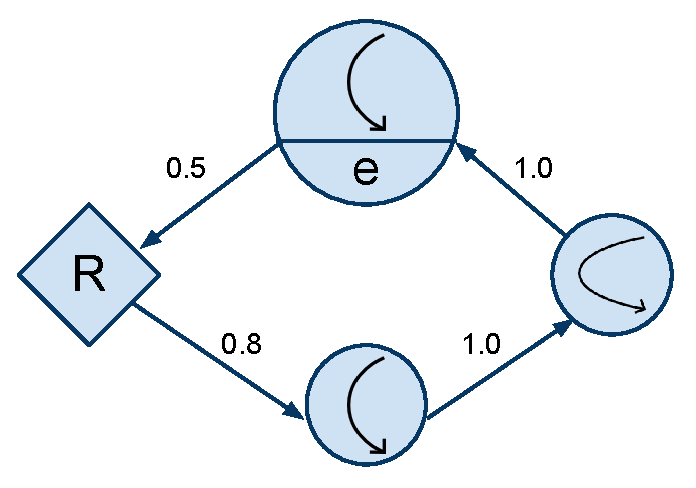
\includegraphics[width=0.5\textwidth]{./img/BeispielGraph.pdf}
  \caption{Ein sehr einfacher Graph für die Erkennung des Buchstaben 'e'}
  \label{beispiel_graph}
\end{figure}

\section{Aufbau}
Der Graph besitzt einen Eintrittspunkt, den \emph{Root-Node}. Von diesem aus wird jeweils die Buchstaben-Erkennung gestartet. Jedes Mal wenn der Pfad auf dem Graph wieder zurück auf den Root-Node führt, bedeutet dies dass die Buchstaben-Erkennung abgeschlossen ist und ein neuer Buchstaben beginnt. 

Die restlichen Nodes beinhalten alle eine bestimmte Mikrogeste und optional ein Zeichen. Ausserdem besitzt der Graph gewichtete Kanten

\section{Erkennungswahrscheinlichkeit}
Jeder Node besitzt eine bestimmte Wahrscheinlichkeit. Beim durchlaufen des Pfades werden alle Wahrscheinlichkeiten multipliziert. So können häufige Mikrogestenn-Abfolgen gestärkt werden und seltene geschwächt. Ausserdem gibt es immer mehrere Möglichkeiten, wie der Graph durchschritten werden kann. Die resultierende Wahrscheinlichkeit gibt ein Indiz dafür, welches Resultat das richtige ist.

\section{Erkennung von Zeichen}

	\part{Lösung}
		% Verschiedene Ansätze beschreiben
		\chapter{Mikrogesten-Erkennung}

Nach der Sichtung der vorgegangen Projektarbeit haben wir uns entschieden, dass zwei Ansätze zur Erkennung der einzelnen Mikrogesten aus der Eingabe-Menge an Punkten im Prototyp ausprobiert und evaluiert werden sollten. Zum einen sollte die in der Projektarbeit favorisierte Erkennung durch die Änderung der Krümmung zwischen den einzelnen Punkten getestet werden, zum Anderen ein Ansatz ausprobiert werden, der auf einer auf dem vorausgehenden Punkt basierenden Voraussage des jeweils als nächstes folgenden Punktes aufbaut.

Der Krümmungs-Ansatz wurde in der vorgängigen Projektarbeit neben einem auf der Änderung der Winkel zwischen Punkten basierenden Ansatz zur Mikrogesten-Erkennung evaluiert und am Ende von den Autoren der Arbeit favorisiert. Dadurch war klar, dass wir diese Art der Erkennung ebenfalls für diese Arbeit evaluieren sollten.

Neben einer Erkennung durch die Krümmungs- und die Winkel-Änderung zwischen Punkten sollte unserer Meinung nach auch eine Erkennung durch die Voraussage von folgenden Punkten möglich sein und wurde daher von uns ebenfalls implementiert und evaluiert.

Diese Ansätze bewährten sich für die Variante A der Mikrogesten, jedoch gab es gewisse Schwierigkeiten, die Mikrogesten der Variante B zu erkennen. Um Spezialfälle wie z.B. einen Kreis zu erkennen, haben wir zusätzliche Algorithmen entwickelt, die nur eine sehr spezialisierte Aufgabe erfüllen. So gibt es zum Beispiel einen Algorithmus, der nur Linien erkennt und einen, der nur Halbkreise erkennt.

\section{Bewertungs-Kriterien}

\begin{table}[h!]
  \begin{center}
    \begin{tabular}{ m{2.2cm} |  p{10cm} }
    \emph{Kriterium} & Erkennungszuverlässigkeit  \\ \hline
    \emph{Beschreibung} & Um eine verlässliche Erkennung der Mikrogesten zu ermöglichen, muss ein Ansatz natürlich gewährleisten, dass er die Auftrennung der Mikrogesten zuverlässig vornimmt. \\ \hline
    \emph{Priorität} & Primär  \\
    \end{tabular}
  \end{center}
  \caption{Kriterium Erkennungszuverl\"{a}ssigkeit}
  \label{kriterium_erkennungszuverlaessigkeit}
\end{table}

\begin{table}[h!]
  \begin{center}
    \begin{tabular}{ m{2.2cm} |  p{10cm} }
    \emph{Kriterium} & Toleranz  \\ \hline
    \emph{Beschreibung} &

 Obwohl die Erkennung natürlich zuverlässig sein sollte, muss aber auch eine gewisse Toleranz für nicht ideale Eingaben gewährt werden. Da die Handschriften-Erkennung auf Menschen und einen Einsatz im mobilen Umfeld ausgerichtet werden soll, sind suboptimale Eingabefolgen durchaus zu erwarten und die Erkennung der Mikrogesten sollte daher einigermassen tolerant auf solche reagieren. Dies stellt offensichtlich ein Zielkonflikt zum Zuverlässigkeits-Kriterium dar und es muss daher ein guter Mittelweg zwischen diesen beiden Kriterien gefunden werden. 
\\ \hline
    \emph{Priorität} & Primär  \\
    \end{tabular}
  \end{center}
  \caption{Kriterium Toleranz}
  \label{kriterium_toleranz}
\end{table}

\begin{table}[h!]
  \begin{center}
    \begin{tabular}{ m{2.2cm} |  p{10cm} }
    \emph{Kriterium} & Performanz  \\ \hline
    \emph{Beschreibung} &

 Auf einem mobilen System ist der schonende Umgang mit den Systemressourcen besonders wichtig und das Verfahren zur Erkennung der Mikrogesten sollte daher möglichst wenig Rechenleistung brauchen. Da es allerdings nur jeweils nach Benutzereingaben durchgeführt werden muss und eine Ausführung im Hintergrund möglich sein sollte, könnten gewisse Abstriche in diesem Bereich unter Umständen in Kauf genommen werden.
\\ \hline
    \emph{Priorität} & Sekundär  \\
    \end{tabular}
  \end{center}
  \caption{Kriterium Performanz}
  \label{kriterium_performanz}
\end{table}

%================================================
\section{Verfahren zur Auftrennung des Pfades}
\subsection{Ansatz: Punkte-Voraussage}
%TODO Ev. diesen Satz etwas einfacher formulieren
Grundlage des auf Voraussage des jeweils nächsten Punktes basierenden Ansatzes sollte die Annahme sein, dass man den als nächstes auf einen Punkt einer gleichmässig gekrümmten Kurve folgenden Punkt durch das Spiegeln des jeweils dem Ausgangspunkt vorangehenden Punktes an der Achse des Ausgangspunktes vorherbestimmen können müsste. Weicht der tatsächlich eingegebene Folgepunkt zu sehr vom vorausgesagten Folgepunkt ab, sollte nun angenommen werden, dass dieser Punkt nicht mehr zur aktuellen Mikrogeste gehören und als Ausgangspunkt einer neuen Mikrogeste genommen werden soll.


\subsubsection{Bewertung}
Die grundsätzliche Trennung der einzelnen Mikrogesten durch das auf Voraussagen basierende Verfahren wurde von uns als durchaus zufriedenstellend bewertet. Das Verfahren ermöglicht die Auftrennung der Eingabepunkte in verschiedene Mikrogesten. Allerdings erkennt das Verfahren unserer Meinung nach leider zu viele einzelne Mikrogesten und ist zu wenig tolerant gegenüber kleineren Abweichungen. Schon kleinere Änderungen in der Linienführung führen dabei zu einer Auftrennung von ansonsten durchaus zusammenhängenden Gesten.

Auch weist das Verfahren Probleme mit ungleichen Punktedichten auf einem Pfad auf. Dies tritt vor allem auf, wenn die Eingabegeschwindigkeit variiert, etwa wenn nach einer Richtungsänderung oder am Anfang einer Geste die Eingabe beschleunigt wird und die späteren Eingabepunkte weiter auseinander liegen als die ersten. Gerade bei unregelmässigen Beschleunigungen kommt es somit häufig vor, dass die ersten Eingabepunkte relativ nahe beieinander liegen, der Abstand zu späteren Punkten dann aber recht gross wird. Die vorausgesagten Punkte mögen dann zwar durchaus auf dem Pfad der Geste liegen, die Eingabepunkte folgend dann allerdings erst in grösserem Abstand. Diesem Verhalten könnte möglicherweise mit Anpassungen an der Berechnung der vorausgesagten Punkte begegnet werden. Man könnte etwa anstatt eines konkreten Punktes eine Richtung voraussagen. Auch ein normierter Abstand zwischen den Eingabepunkten, wie ihn das Spline-Glättungsverfahren erzeugt, welches als mögliche Optimierung in \ref{sec:Glaettung} besprochen wird. Eine Glättung der Eingangspunkte sollte auch die Toleranz des voraussagenden Ansatzes verbessern können.

Weiter haben wir mit diesem Verfahren Probleme mit zu nahe beieinander liegenden Eingabepunkten festgestellt. Ist die Distanz von einem Punkt zum nächsten kleiner als die Länge des Toleranz-Wertes, fällt der Punkt in jedem Fall innerhalb der Toleranz und es kann keine fundierte Aussage über mehr darüber gemacht werden, ob der Punkt zur selben Mikrogeste gehören soll oder nicht. Daher werden nur Punkte, deren Abstand zum Ausgangspunkt kleiner als die zweifache Länge des Toleranz-Wertes sind, beachtet. Andere Punkte werden als zur aktuellen Mikrogeste gehörig angenommen und zum neuen Ausgangspunkt. Dies führt wiederum zu Problemen mit sehr engen Kurven, wie sie etwa bei Richtungswechseln und sehr eng-winkligen Spitzen, da diese eng beieinander liegende Eingabepunkte erzeugen, deren Abstand häufig unterhalb die Toleranzgrenze fällt. Somit wird häufig noch der erste Punkt nach einer solchen Spitze zur vorherigen Mikrogeste zugeordnet.

Diesen beiden Probleme, welche beide das als substantiell gewertete Bewertungskriterium der Toleranz beeinträchtigen, steht steht nur eine gute Performanz durch die relativ simplen Berechnungen, die das Voraussage-Verfahren benötigt, gegenüber. Da das Toleranz-Kriterium von uns aber als signifikant wichtiger eingestuft wurde und vom Krümmungs-Verfahren weit besser erfüllt wird, mussten wir uns am Ende für das auf Krümmungs-Änderungen basierende Verfahren festlegen.

%================================================

\subsection{Ansatz: Krümmungs-Änderung}
Das Krümmungsverfahren basiert auf dem Verfahren, das in \cite{zeichenerkennung_pa} vorgeschlagen wird: Die Punkte eines Pfades werden mit Vektoren verbunden. Zwischen jedem Vektor und seinem Nachfolger wird nun das Kreuzprodukt (siehe Abbildung \ref{kreuzprodukt}) gebildet. Das Vorzeichen des Resultats gibt nun die Drehrichtung der Kurve an. Die Änderung der Drehrichtung ist bereits eine wichtige Information um den Pfad in Mikrogesten zu unterteilen.
Als zweite Information erhält man den Winkel zwischen den Vektoren. Nun kann man den Pfad an den Stellen trennen, wo der Winkelunterschied zu den vorherigen Vektoren eine gewisse Toleranz überschreitet. Dies ist vor allem nützlich um zwischen einer starken und einer schwachen Krümmung zu unterscheiden.

\begin{figure}[h!]
  \centering
    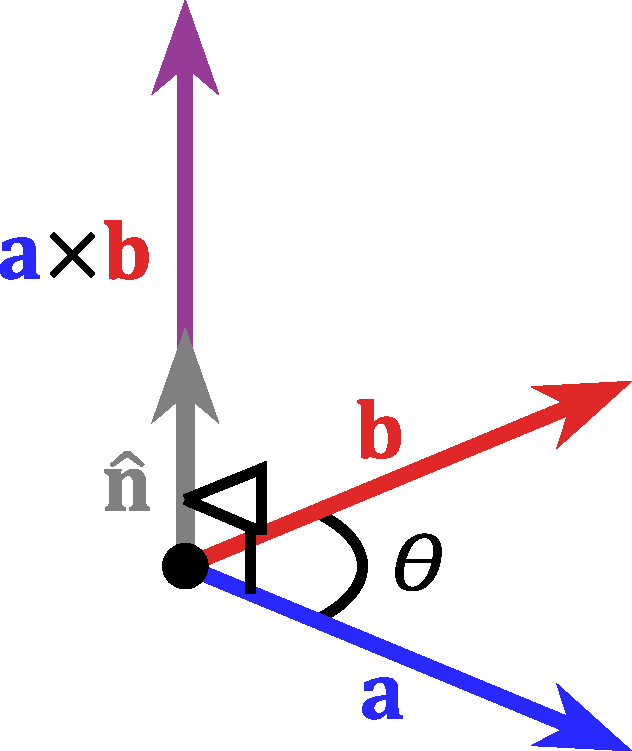
\includegraphics[width=0.3\textwidth]{./img/crossproduct.pdf}
  \caption{Kreuzprodukt zweier Vektoren}
  \label{kreuzprodukt}
\end{figure}

\subsubsection{Verfahren}
Das Vorgehen bei diesem Algorithmus ist sehr simpel: Es wird laufend die Krümmung zwischen dem aktuellen Punkt und seinen Nachbarn berechnet. Sobald die Krümmung einen gewissen Toleranzwert überschreitet wird der Pfad in zwei Mikrogesten aufgetrennt. Der genaue Ablauf ist in Abbildung \ref{curvatureflowchart} ersichtlich.

\begin{figure}[h!]
  \centering
    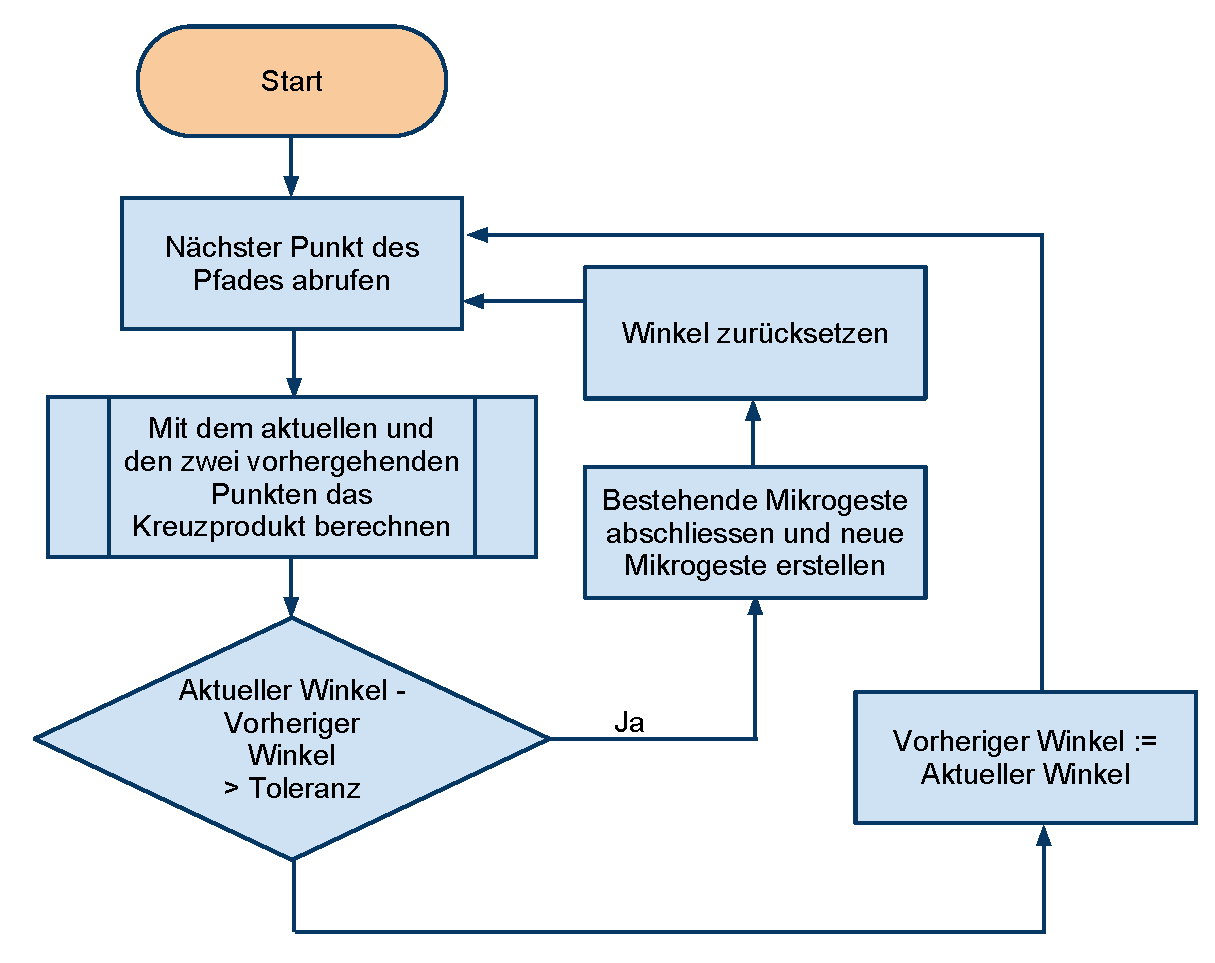
\includegraphics[width=\textwidth]{./img/CurvatureFlowchart.pdf}
  \caption{Ablauf des Krümmungs-Algorithmus}
  \label{curvatureflowchart}
\end{figure}

\subsubsection{Bewertung}
Das Verfahren is vor allem gut geeignet um Änderungen in der Drehrichtung zu erkennen (Nützlich z.B. bei dem Buchstaben 'S') und zwischen starken und schwachen Krümmungen zu unterscheiden. Es hat allerdings die gleichen Probleme wie die Punkte-Voraussage: Die Eingangspunkte müssen gut normiert sein um gleichmässige Erkennung zu garantieren. Dieses Problem kann jedoch mit einer Vorbearbeitung des Pfades gelöst werden.

%================================================

\subsection{Ansatz: Drehrichtungs-Erkennung}
Dieser Ansatz ist eine Abwandlung des Krümmungs-Verfahrens und so abgeändert, dass Drehrichtungsänderungen möglichst genau erkannt werden können. Der Hintergedanke dabei ist dass man bei Mikrogesten nur noch zwischen Kurven unterscheidet, die in eine andere Richtung drehen, aber nicht mehr die Stärke der Krümmung berücksichtigt.

\subsubsection{Verfahren}
Das Verfahren funktioniert prinzipiell gleich wie das Krümmungs-Verfahren: Es wird immer für zwei benachbarte Vektoren das Vektorprodukt berechnet. Der errechnete Wert wird immer zu einem Akkumulator addiert und mit dem Punkt abgespeichert. Nach dem der komplette Pfad so durchgerechnet wurde, erhält man eine Akkumulator-Kurve. In Abbildung \ref{drehrichtungsBeispiel} ist eine Beispiel-Eingabe gezeigt und in Abbildung \ref{akkumulatorDiagramm} der dazu berechnete Akkumulator-Verlauf. Wie man sieht stellen die Maxima und Minima der Kurve die Richtungswechsel in der Eingabe dar. Die Trennungspunkte können also durch ein einfaches berechnen aller lokalen Maxima und Minima bestimmt werden.

\begin{figure}[h!]
  \centering
    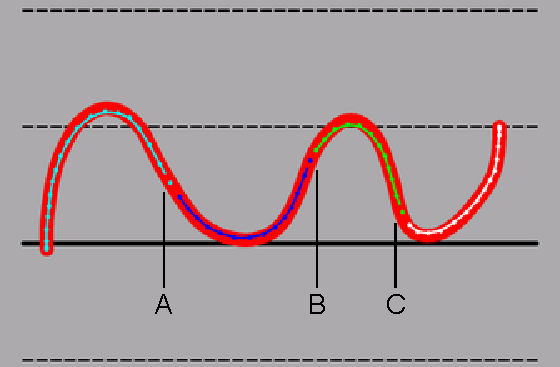
\includegraphics[width=0.67\textwidth]{./img/akkumulator_beispiel.pdf}
  \caption{Beispiel-Eingabe: rot, Erkannte Trennungen: Farbig.}
  \label{drehrichtungBeispiel}
\end{figure}

\begin{figure}[h!]
  \centering
    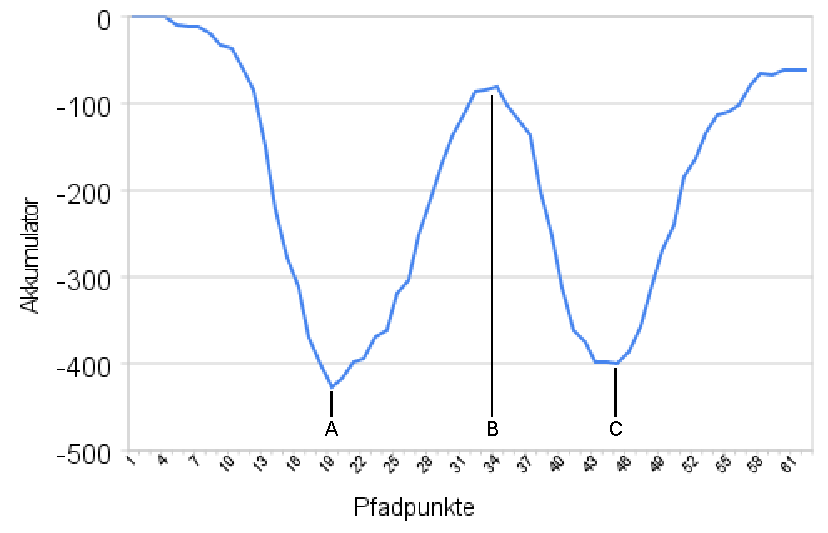
\includegraphics[width=1.0\textwidth]{./img/akkumulator_diagramm.pdf}
  \caption{Akkumulator für die Eingabe von Abbildung \ref{drehrichtungBeispiel}.}
  \label{akkumulatorDiagramm}
\end{figure}

\subsubsection{Bewertung}
Dieser spezialisierte Algorithmus funktioniert sehr gut, wenn der Pfad tatsächlich nur aus Kurven besteht. Deshalb ist es nötig, dass mit einem anderen Algorithmus alle Geraden aus dem Pfad entfernt wurden (Zum Beispiel dem Krümmungsalgorithmus).

%================================================

\subsection{Ansatz: Winkel-Änderung}

Dieses Verfahren funktioniert prinzipiell wie das Krümmungs-Verfahren. Es ist jedoch vereinfacht und berücksichtigt nur noch den Winkel zwischen zwei benachbarten Vektoren.

\subsubsection{Verfahren}
Es wird der Winkel zwischen den Vektoren berechnet und mit der Toleranz verglichen. Bei einem genügend spitzigen Winkel wird der Pfad aufgetrennt. Abbildung \ref{kanten_trennung} zeigt ein Beispiel einer Trennung.

\lstinputlisting [caption={Pseudocode-Algorithmus um scharfe Kanten im Pfad zu erkennen},label=edgesalgorithmus]{code/edges.pseudo}

\begin{figure}[h!]
  \centering
    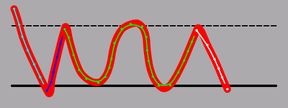
\includegraphics[scale=0.75]{./img/edges_beispiel.png}
  \caption{Beispiel einer Trennung: Jede farbige Linie ist eine erkannte Mikrogeste.}
  \label{kanten_trennung}
\end{figure}

\subsubsection{Bewertung}
Dieses Verfahren ist sehr einfach gehalten und darauf spezialisiert, Spitzkehren im Pfad zu erkennen. Der grosse Nutzen dieses Verfahren ist aber, dass der Pfad nicht normiert werden muss. Die anderen Verfahren erkennen zwar Spitzkehren auch, brauchen aber einen normierten, am besten geglätteten, Pfad. Die Glättung schwächt aber Spitzkehren ab und macht sie ev. sogar unkenntlich.  

%================================================

\subsection{Ansatz: Kreis-Erkennung}
Mit diesem Ansatz sollen alle geschlossenen Kreise auf dem Pfad erkannt werden. Alle restlichen Punkte werden nicht berücksichtigt und müssen mit einem anderen Verfahren aufgetrennt werden.

\subsubsection{Verfahren}
Mit jedem Punkt auf dem Pfad werden alle nachfolgenden Punkte verglichen: Wenn die zwei Punkte sehr nahe beieinander liegen bildet der Pfad zwischen den Punkten ein Kreis.

\lstinputlisting [caption={Pseudocode-Algorithmus um Kreise auf einem Pfad zu erkennen},label=kreisalgorithmus]{code/circle.pseudo}

\begin{figure}[h!]
  \centering
    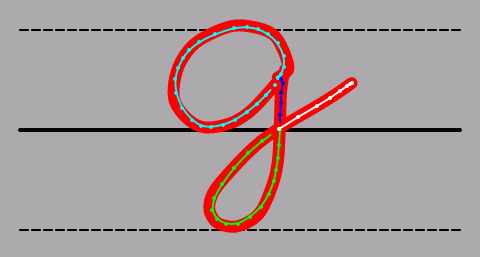
\includegraphics[scale=0.5]{./img/circle_beispiel.png}
  \caption{Beispiel einer Kreiserkennung: Farbige Linien stellen Mikrogesten dar.}
  \label{kreis_trennung}
\end{figure}

\subsubsection{Bewertung}
Die Kreiserkennung ist natürlich nur sinnvoll, wenn man eine entsprechende Mikrogeste "Kreis" hat. Allerdings gibt es auch beim Algorithmus noch Verbesserungsbedarf: Bei einem Spezialfall, nämlich ein Pfad der eine '8' bildet, wird der gesamte Pfad als ein Kreis erkannt und nicht als zwei Kreise. 


%================================================
\subsection{Fazit}
Es hat sich gezeigt, dass es nicht sinnvoll ist, sich auf ein einzelnes Verfahren zu stützen. Jedes Verfahren hat seine Schwächen, welche von einem anderen Verfahren abgedeckt werden können. Es ist am besten, den Pfad schrittweise zu unterteilen und bei jedem Schritt die Mikrogesten-Erkennung zu starten. Mit jedem weiteren Schritt werden dann nur noch Pfadteile berücksichtigt, welchen noch keine Mikrogeste zugewiesen ist.

%================================================

\section{Erkennung der Mikrogesten-Art}
Die Erkennung der Mikrogeste kann je nach Form der Mikrogeste unterschiedlich aufwändig sein. Deshalb haben wir für beide Mikrogesten-Varianten eigene Erkennungsalgorithmen erstellt:

\subsection{Variante A}
%% TODO sollte noch etwas erweitert werden
Für diese Variante ist die Unterscheidung von Line, schwacher Krümmung und starker Krümmung nötig. Die Erkennung ist deshalb recht einfach: Die Stärke der Krümmung unterscheidet alle Mikrogesten voneinander.

\subsubsection{Kreisradius berechnen}
Ein einfaches Verfahren zur Kategorisierung ist folgendes: Es wird mit einem Kreis die Punktemenge der Mikrogeste angenähert. Mit dem Radius dieses Kreises kann dann die Art der Geste bestimmt werden:
\begin{itemize}
\item \emph{Kleine Radien:} Starke Krümmung
\item \emph{Unendlich grosse Radien:} Linie
\item \emph{Rest:} Schwache Krümmung
\end{itemize}

\subsection{Variante B}
%% TODO MIt einem Flussdiagramm beschreiben
Für diese Variante läuft die Erkennung in mehreren Schritten ab:
\begin{enumerate}
\item Es werden mit dem Kreis-Algorithmus alle Kreise bestimmt.
\item Danach werden von den restlichen Mikrogesten die Geraden bestimmt. Dies wird sichergestellt, indem vom ersten zum letzten Punkt eine Linie gezogen wird. Wenn kein Punkt der Mikrogeste zu stark von der Linie abweicht, ist die Mikrogeste eine Gerade.
\item Alle übrigen Mikrogesten sind nun entsprechend automatisch Kurven.
\end{enumerate}

Diese Schrittweise Erkennung ist notwendig, da nach jedem Erkennungsschritt die übrigen Pfadteile in weitere Mikrogesten aufgeteilt werden.

%================================================

\section{Erkennung der Ausrichtung einer Mikrogeste}
Für jede Mikrogeste muss auch die Richtung bestimmt werden. Im Endeffekt gibt es nur vier verschiedene Richtungen, wie im theoretischen Teil beschrieben. 
\subsubsection{Richtung der Gerade}
Die Richtungsbestimmung einer Geraden ist sehr simpel, da die Steigung der Geraden direkt die Richtung darstellt.
\subsubsection{Richtung der Krümmungen}
Hier wird eine Gerade an die Krümmung approximiert und so die Richtung bestimmt.
\subsubsection{Richtung der Halbkreise}
%% TODO mit einem Diagramm darstellen
Für die Halbkreise ist die Richtungs-Bestimmung etwas schwieriger. Hier wird bestimmt, in welche Richtung die Öffnung zeigt.
Dazu wird zuerst bestimmt, ob die Öffnung oben/unten oder links/rechts ist. Wenn beide Endpunkte in etwa gleiche y-Werte haben ist die Öffnung oben/unten, wenn sie etwa gleiche x-Werte haben ist die Öffnung links-rechts.
Um zu bestimmen ob die Öffnung nun oben oder unten ist, muss nur die Anzahl der Punkte bestimmt werden, deren y-Werte unter denen der beiden Endpunkte liegt. Liegen die meisten Punkte darunter, ist die Öffnung nach oben, sonst nach unten. Für links und rechts kann gleich verfahren werden, einfach mit den x-Werten.

%================================================

\section{Allgemeine Optimierungen}

\subsection{Normierung der Eingangspunkte}
%%TODO Diagramm dazu
Eine Normierung der Eingangspunkte ist nötig, um immer gleiche Voraussetzungen für die Algorithmen zu garantieren. Der durchschnittliche Abstand zwischen den Punkten, die beim schreiben vom Touchpad erfasst werden, ist hauptsächlich von der Schreibgeschwindigkeit, aber auch von der Qualität des Touchpads abhängig. 

\lstinputlisting[caption={Algorithmus zur groben Normierung der Eingangspunkte},label=normierung_algorithmus]{code/normierung.pseudo}

\subsection{Zusammenfügen von minimalen Mikrogesten}
Die Mikrogesten-Algorithmen erstellen manchmal sehr kurze (nur ganz wenige Punkte) Mikrogesten. Da sie so kurz sind, sagen sie auch nicht wirklich etwas über die Form des eingegebenen Zeichen aus. Dies kann optimiert werden, indem die Punkte einfach der vorhergehenden Mikrogeste angehängt werden und die kurze Geste verworfen wird.

\subsection{Glättung der Eingangspunkte}\label{sec:Glaettung}
Für die Erkennung der Mikrogesten ist es von Vorteil, dass der Buchstaben relativ ``rund'' eingegeben wurde und nicht zu sehr verwackelt. Dies würde sonst zu einer Erkennung von mehreren kurzen Mikrogesten führen, wo eigentlich nur eine einzige, zittrige Mikrogeste gemacht wurde. Mit einem Glättungs-Algorithmus kann der Pfad zusätzlich optimiert werden. 

Für die Glättung verwenden wir \emph{rational B-Splines} \cite[S. 454]{smoothing_book} da diese Perfekt für Pfad-Glättung konzipiert sind. Allerdings muss beachtet werden, dass gewisse Kanten im Pfad gewünscht sind, wie zum Beispiel Spitzkehren. Eine Glättung würde diese Merkmale abschwächen und die Erkennung damit verschlechtern. Es ist deshalb von Vorteil wenn nur die Teilpfade zwischen solchen gewünschten Kanten geglättet wird.

Ein nützlicher Nebeneffekt der Splines ist, dass die Resultierende Kurve aus einer beliebig gewählten Anzahl Punkten besteht. Diese Punkte sind bereits gleichmässig verteilt. Eine Punktenormierung ist deshalb durch die Spline-Glättung auch schon durchgeführt.

%%TODO: Zusammenfügen von identischen nacheinander folgenden Mikrogesten
%================================================

\section{Vergleich der Ansätze}
Es zeigt sich, dass die Algorithmen sehr stark darauf optimiert werden können, wie die Mikrogesten genau aussehen. Für die Variante A, wo die Krümmung der Hauptunterschied zwischen den Mikrogesten ist, funktioniert auch die trennung nach Krümmung am besten.

Ein sehr grosses Problem ist hingegen die Toleranz der Algorithmen: Das Ziel wäre es, bei ungefähr gleicher Eingabe immer die gleichen Mikrogesten zu erhalten. Es hat sich jedoch gezeigt, dass dies kaum zu erreichen ist. Gerade bei der Variante A mit den Krümmungen kann es bei der Eingabe eines Buchstabes jedes Mal eine andere Mikrogesten-Folge erkennen. 

Das ist auch der Grund weshalb wir einen zweiten Ansatz entwickelt haben: Man muss Mikrogesten verwenden, die bei unterschiedlicher Schreibweise trotzdem noch erkennbar sind. Der Kreis ist das Paradebeispiel dafür: Es muss nur ein geschlossener Pfad vorhanden sein, egal welche Form er hat. Ausserdem haben wir die Idee verworfen, verschieden starke Krümmungen zu unterscheiden. Das ist zwar sehr einfach umzusetzen, kann aber von Schreibstil zu Schreibstil sehr stark variieren. Einzig ein Richtungswechsel führt noch zu einer neuen Mikrogeste, da dies in den allermeisten Fällen vom Schreibenden auch gewollt gemacht wurde.

Anschliessend deshalb die Vorgehensweisen für beide Varianten:

\subsection{Vorgehen Variante A}
\begin{enumerate}
	\item Normierung der Punktezahl: Zu nahe beieinander liegende Punkte werden gelöscht. Bei zu grossen Abständen wird zwischen den zwei Punkten interpoliert.
	\item Unterscheidung von verschieden starken Krümmungen
	\item Bestimmung der Krümmungsstärke ergibt Mikrogesten-Typ
\end{enumerate}

Bei diesem Ansatz ist zwar die Erkennungszuverlässigkeit gegeben, allerdings nützt dies nichts, da die Mikrogesten-Typen überhaupt nicht tolerant gegenüber anderen Schreibstilen sind. Es ist zwar möglich, dies im Graph zu kompensieren, dies erhöht jedoch auch wieder die Wahrscheinlichkeit, dass es zu Überschneidungen zwischen verschiedenen Buchstaben kommt.

\subsection{Vorgehen Variante B}
Der Ansatz ist wie folgt:
\begin{enumerate}
	\item Normierung der Punktezahl: Zu nahe beieinander liegende Punkte werden gelöscht. Bei zu grossen Abständen wird zwischen den zwei Punkten interpoliert.
	\item Erkennung der spitzen Winkel im Pfad.
	\item Glättung des Pfades
	\item Erkennung aller geschlossenen Kreise 
	\item Unterteilung in Kurven und Geraden
	\item Unterteilung der Kurven bei Drehrichtungswechsel
\end{enumerate}

Die Erkennungszuverlässigkeit ist für diesen Ansatz relativ gut: Bloss bei der Erkennung der Halbkreis-Richtung gibt es noch Spezialfälle, die nicht unbedingt korrekt erkannt werden. Dies liegt daran, dass natürlich nicht alle Kurven perfekte Halbkreise bilden. Die Toleranz ist dafür im Vergleich zu Variante A einiges besser. Dies wird auch durch die Glättung erreicht, die den Pfad verbessert. Da die scharfen Kanten vor der Glättung erkannt werden, gibt es dort auch keine Verschlechterung des Resultats. Die Erkennung von Kreisen funktioniert auch sehr tolerant, da die Form des Pfades nicht berücksichtigt wird. Einzig bei den Geraden kann es noch Probleme geben: Es kommt manchmal vor, dass statt einer Langen Gerade mehrere kurze Geraden erkannt werden. Diese Problem kann noch mit einer intelligenten Kombination von kurzen Geraden gelöst werden.

		

		\chapter{Zeichen-Erkennung}

\section{Vergleich der Ansätze}
\section{Probleme \& Lösungsvorschläge}

		\chapter{Backend}

Bevor wir zur Besprechung der Umsetzung des eigentlichen Backends übergehen, wollen wir zuerst einige grundsätzliche Überlegungen zur Art des Prozesses, den wir für unser Backend einsetzen wollen, festhalten.

\section{Art des Prozesses}

\subsection{Prozesse unter Android}

Da in der Entwicklung für das Android-Betriebssystem ein etwas erweitertes Vokabular für die Beschreibung des Applikations-Lebenszyklus verwendet wird, wollen wir zuerst kurz auf einige dieser Begriffe im Android-Kontext eingehen.

Applikationen laufen unter Android grundsätzlich in einem eigenen Thread den das Betriebssystem als separaten Linux-Prozess startet und werden auch vom Betriebssystem wieder beendet. Sollen Komponenten in einem eigenen Prozess laufen, können weitere Threads gestartet werden\cite{adglc}. Diese können über die standard Thread-Objekte von Java erzeugt werden, werden aber mit dem Applikations-Prozess terminiert, sollte Android entscheiden dass dieser nicht mehr benötigt wird. Um dies, wenn Ressourcen benötigt werden sollten, möglich effizient durchzuführen, werden Prozesse vom Betriebssystem einfach abgewürgt (ein kill-Signal wird gesendet) und keinerlei Aufräumfunktionen werden ausgeführt. Applikationen sind daher selbst dafür verantwortlich, ihren Status zu sichern, wenn sie in den Hintergrund geschickt werden\cite{adbmt}.

Unser Erkennungs-Backend sollte nun aber auch unabhängig vom Frontend weiterlaufen. Grundsätzlich wäre das beenden des Backend-Threads beim Schliessen des Frontends kein grösseres Problem, da wir davon ausgehen können, dass eventuell erst nach Beendung des Frontend-Threads eintreffende Resultate für den Benutzer nicht mehr relevant sind und verworfen werden können bzw. nicht mehr fertig gerechnet werden müssen. Allerdings wäre es zu bevorzugen, wenn bei einem erneuten Aufruf des Frontends der Backend-Thread schon im Speicher vorhanden ist und nicht noch neu initialisert werden muss. Die Initialisierung des Backends kann je nach verwendeter Erkennungs-Methodik recht aufwendig sein. So muss etwa bei der Graphen-Methode zuerst die XML-Datei, in welcher der Graph gespeichert ist, eingelesen und der Graph aufgebaut werden. Der Benutzer erwartet möglichst schnell mit der Eingabe beginnen zu können und eine Initialisierung bei jeder Versuch dazu sollte ihm daher nicht zugemuted werden.

Neben den normalen Threads aus Java kennt Android noch spezialisierte Prozesse, die unabhängig von der Ursprungs-Applikation weiterlaufen können. Für uns interessant sind hier vor allem die Services und die Broadcast-Receiver.

\subsubsection{Broadcast-Receiver}

Broadcast-Receiver werden hauptsächlich dazu verwendet, im Hintergrund auf Ereignisse zu reagieren. Die Handhabung diese Ereignisses durch den Receiver muss innerhalb einer gegebenen Zeit erfolgen\footnote{Im Moment beträgt die zur Verfügung stehende Zeit 10 Sekunden, danach kann der Prozess jederzeit abgewürgt werden\cite{adbmt}}, wodurch diese nur im Speicher gehalten werden müssen, wenn ein solches Ereigniss eintrifft. Broadcast-Receiver sind daher also gut geeignet um kurze Arbeiten als Reaktion auf eine externen Stimulus durchzuführen und werden etwa benutzt um auf Alarme oder Positions-Änderungen zu reagieren. Da sie aber nach Beendigung ihrer Aufgabe voraussichtlich wieder terminiert werden, würden sie für unseren Backend-Prozess keinen Vorteil darstellen, da sich die Frage der Reinitialisierung ebenfalls wieder stellen würde.

\subsubsection{Services}

Services sind unter Android sehr vielseitig und durch sie können Applikationen langlaufende Operationen im Hintergrund ausführen. Grundsätzlich ist ihre Laufzeit nicht beschränkt und ihr Verhalten in dieser Zeit wird weitestgehend von der Applikation bestimmt. So können sie etwa vom restlichen Programm unabhängige Operationen ausführen, auf gemeinsame Singelton-Objekte zugreifen oder gar in einen eigenen Prozess ausgelagert werden.

Services können allerdings vom Betriebssystem jederzeit abgeschossen werden, wenn es Ressourcen benötigen sollte. Allerdings wird sich Android merken, wenn es Services, die weiter laufen wollen, terminiert. Wenn wieder genug Arbeitsspeicher verfügbar ist, werden die beendeten Services wieder neu gestartet. Auch ist es möglich, dass Services beantragen, als Vordergrund-Prozesse behandelt zu werden und so recht gut vor dem Terminieren geschützt sind. Dies muss dem Benutzer allerdings angezeigt werden, damit sich dieser des laufenden Prozesses bewusst ist.

Für unser Backend sollte ein Service also die am besten geeignete Prozess-Form sein, da wir den Backend-Service im Hintergrund weiter laufen lassen können, nachdem eine Eingabe getätig wurde. Eine Terminierung bei zu wenig vorhandenem Speicher können wir akzeptieren, da der Service danach wieder neu gestartet werden sollte und die Initialisierung vom Benutzer unbemerkt im Hintergrund stattfinden kann. Wir benötigen daher auch nicht die Privilegien eines Vordergrund-Prozesses.
%================================================

\section{Analyse}

\subsection{Initialisierung}

\subsection{Ablauf der Erkennungs}

Um den Ablauf der Erkennung möglichst flexibel zu machen, wurde dieser in mehrere Phasen aufgeteilt. Einige dieser Phasen sollen wiederum in mehrere Einzelschritte aufgeteilt werden.

\begin{figure}[h]
   \centering
   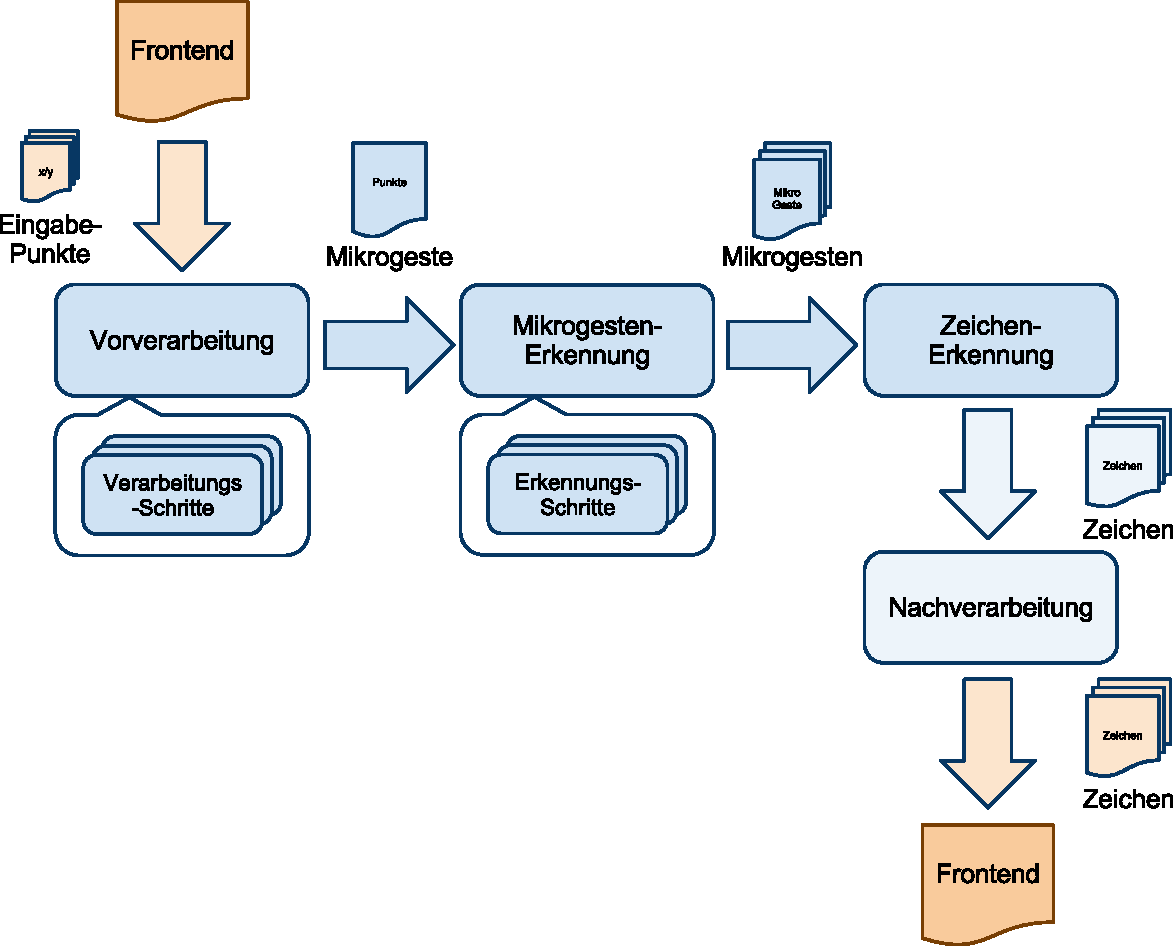
\includegraphics[scale=0.75, bb=10 0 744 460]{img/erkennungs_ablauf.pdf} 
   \caption{Erkennungs-Ablauf}
   \label{fig:erkennungs_ablauf}
\end{figure}

Zuerst soll eine Vorverarbeitung der Eingabe-Punkte durchgeführt werden, in der etwa eine Normierung, eine Glättung, eine Filterung oder ähnliches dieser durchgeführt werden kann. Diese Verarbeitungs-Schritte sollen sich nicht gegenseitig ausschliessen, sollen aber auch optional sein, da einige der dazu möglichen Algorithmen sehr rechenaufwendig sind.

Die zweite Phase soll die Erkennung der Mikrogesten sein. Auf diese soll in mehrere Erkennungs-Schritte aufgeteilt sein, die gegebenenfalls auch deaktiviert werden können.

Als nächstes soll die Zeichen-Erkennung durchgeführt werden. Diese soll allerdings in sich geschlossen funktionieren und nicht zwingend weiter in Teil-Schritte aufgeteilt werden. Das Erkennungs-Verfahren als ganzes soll allerdings austauschbar sein.

Die vierte und letzte Phase soll die Nachverarbeitung der erkannten Zeichen sein. Dies kann etwa bedeuten, das gewisse Zeichen wieder verworfen werden oder das die Gewichtung der Erkennungs-Wahrscheinlichkeit der Zeichen angepasst wird.

\subsubsection{Vorverarbeitung}

\subsubsection{Mikrogesten-Erkennung}

\subsubsection{Zeichen-Erkennung}

\subsubsection{Nachverarbeitung}
%================================================

\section{Design}

(Klassendiagramm, Sequenzdiagramm)
%================================================

\section{Implementation}

(...)
%================================================



	\part{Evaluation}
		\chapter{Vergleich der Varianten A und B}
Wir haben bereits einige Vor- und Nachteile der einzelnen Mikrogesten-Varianten diskutiert und möchten nun den tatsächlichen Unterschied praktisch testen. Für beide Varianten wird  ein Graph verwendet, um mit den Mikrogesten einen Buchstaben zu erkennen. Da der Graph sehr starr ist, muss die Mikrogesten-Erkennung bei jeder Eingabe eines Buchstaben das gleiche Resultat ergeben. Im Endeffekt besteht der Unterschied der beiden Varianten nur in der Mikrogesten-Erkennung.

\section{Vorgehensweise}
Die Varianten wuren folgendermassen verglichen:
\begin{itemize}
\item Wahl beliebiger Buchstaben.
\item Jeden Buchstaben theoretisch mit den beiden Varianten aufbauen.
\item Den Buchstaben 20x für jede Variante eingeben und die erkannten Mikrogesten loggen.
\item Die erkannten Mikrogesten mit den theoretischen vergleichen und die prozentuale Übereinstimmung errechnen
\item Den Mittelwert über alle Versuche berechnen. Dieser Wert kann dann zum Vergleich verwendet werden.
\end{itemize}

\section{Resultate}
Die kompletten in den Tests gewonnenen Daten sind im Anhang \ref{anhang_vergleich} zu finden. In den folgenden Abschnitten werden die Resultate jedoch noch untersucht und erläutert.

\subsection{Buchstabe 'm'}
Der Buchstabe 'm' lässt sich in beiden Varianten mit relativ wenigen Mikrogesten abbilden. In der Variante B kann dieser zum Beispiel aus nur drei Mikrogesten aufgebaut werden. Dies führt dazu, dass bei einer falsch erkannten Mikrogeste die Erkennungsrate schon drastisch sinkt. Im Gegenzug ist aber auch die Wahrscheinlichkeit höher, eine perfekte Erkennung zu erzielen.

In der Abbildung \ref{test_m} sind die Resultate der Testreihe abgebildet. Dort sieht man auch die starken Schwankungen der Erkennungsrate. In Tabelle \ref{test_avg} sind noch die Mittelwerte festgehalten: Es zeigt sich, dass Variante B trotz einiger schlechter Werte im Schnitt eine bessere Erkennung bietet.

\begin{figure}[h!]
  \centering
    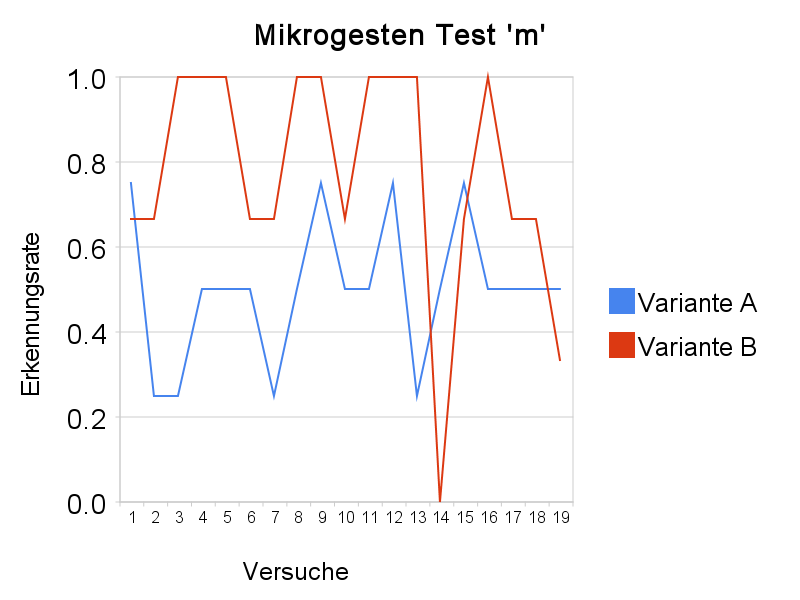
\includegraphics[scale=0.4]{./img/mikrogesten_test_m.png}
  \caption{Resultat der Versuchsreihe mit dem Buchstaben 'm'.  }
  \label{test_m}
\end{figure}

\begin{table}[h!]
  \begin{center}
    \begin{tabular}{l | c |  c }
    \emph{Buchstabe} &  \emph{Variante A} &  \emph{Variante B} \\ \hline
    m & 51\% & 78\% \\ \hline
    k & 45\% &  88\% \\
    \end{tabular}
  \end{center}
  \caption{Durchschnittliche Erkennungsrate der beiden Versuche}
  \label{test_avg}
\end{table}

\subsection{Buchstabe 'k'}
In diesem Test wurde die Erkennungsrate des Buchstaben 'k' in kursivschreibweise getestet. Dies ist der Buchstaben, der aus den meisten Mikrogesten aufgebaut wird und deshalb auch der komplexeste ist. 

Die mittlere Erkennungsrate ist in Tabelle \ref{test_avg} festgehalten und die einzelnen Werte in Abbildung \ref{test_k}. Interessanterweise schneidet der komplexe Buchstabe 'k' besser ab als der einfache Buchstabe 'm'. Dies kann wie folgt erklärt werden: Es gibt eine Reihe von einfachen Buchstaben, die alle aus zwei bis vier Mikrogesten bestehen. Man kann also im Graph nicht viele Varianten eines einzelnen Buchstabens zulassen, da ansonsten schnell Überschneidungen mit anderen Buchstaben entstehen. Wenn nun schon nur eine einzige Mikrogeste falsch erkannt wurde, kann dies bereits zu einem falschen Resultat führen.

Komplexe Buchstaben hingegen unterscheiden sich im Mikrogesten-Aufbau stark von den anderen Buchstaben. Dadurch kann man selbst noch den korrekten Buchstaben finden, wenn einige der Mikrogesten nicht übereinstimmen.

Bei Variante A schneidete 'k' schlechter ab als 'm', was daran liegt, dass die kursive Version von 'k' sehr viele mögliche Schreibweisen besitzt. Da Variante A zwischen starken und schwachen Krümmungen unterscheidet, ist es bei diesem Buchstaben relativ  zufällig, ob jetzt eine starke oder eine schwache Krümmung erkennt wird. Durch den oben genannten Effekt der komplexen Buchstaben ist eine Erkennung aber trotzdem noch möglich.

\begin{figure}[h!]
  \centering
    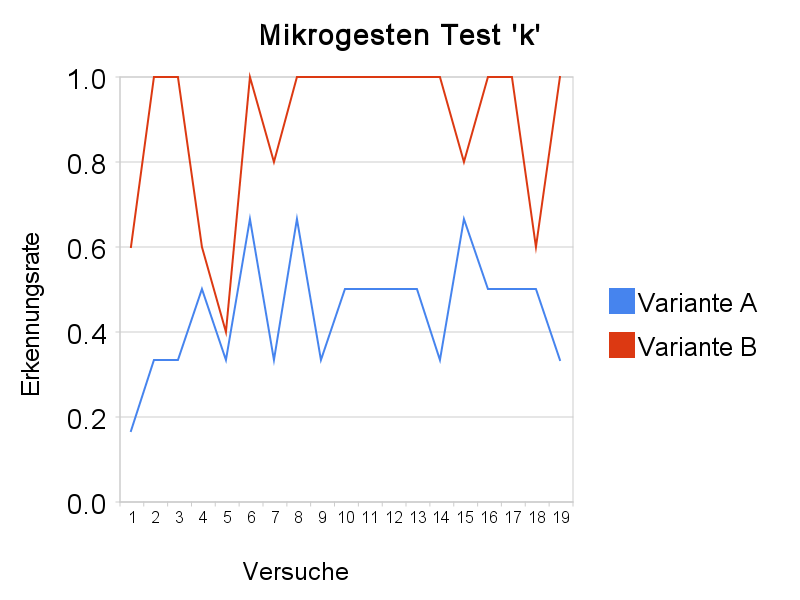
\includegraphics[scale=0.4]{./img/mikrogesten_test_k.png}
  \caption{Resultat der Versuchsreihe mit dem Buchstaben 'k'.  }
  \label{test_k}
\end{figure}

\section{Die perfekte Mikrogesten-Variante}
Aus den bisherigen Erkenntnissen und Tests können folgende Schlüsse gezogen werden:

\begin{itemize}
 \item Die Mikrogesten müssen so definiert sein, dass sie mit einem möglichst einfachen Algorithmus erkannt werden können.
 \item Die Mikrogesten müssen sich so stark wie möglich voneinander Unterscheiden. Eine starke Unterscheidung sollte automatisch auch zu einer einfachen Erkennung führen.
 \item Es ist nicht von Vorteil, die Buchstaben mit möglichst wenigen Mikrogesten aufzubauen. Paradoxerweise kann dies die Erkennungsrate verschlechtern.
\item Nach Erfahrungswerten ist eine Mikrogestenzahl von vier bis sechs am besten geeignet. Die Erkennungsrate der Mikrogesten ist jedoch viel wichtiger als die durchschnittlich benötigte Mikrogestenzahl pro Buchstaben!
\end{itemize}

\section{Fazit}
Variante B schneidet bei der Erkennung besser ab, ist jedoch auch nicht perfekt. Vor allem bei den Kleinbuchstaben hat man immer noch das Problem, dass ähnliche Buchstaben schwer zu unterscheiden sind. Die Ähnlichkeit ist allerdings von der Schrift gegeben und lässt sich nicht ändern. Deshalb ist die sinnvollste Optimierung die Überarbeitung der Mikrogesten-Erkennungsalgorithmen. Dort besteht immer noch sehr viel Verbesserungsbedarf: Wie beim Test gesehen, werden selbst einfache Buchstaben nur in 78\% der Fälle erkannt.
		
		\chapter{Verbesserungsmöglichkeiten}
Unsere Lösung für das Problem besitzt noch einiges an Verbesserungspotential. In diesem Kapitel werden wir einige Ideen aufzeigen, die wir aus Zeitgründen nicht mehr umsetzen konnten.

\section{Mikrogesten-Erkennung}


\section{Zeichen-Erkennung}
\subsection{Neuronales Netz}
Als Alternative zum Graphen bietet isch ein neuronales Netz an. Es gibt bereits speziell auf Handschrifterkennung ausgerichtete neuronale Netze zum Beispiel von Microsoft. Das spezielle an diesen Netzen ist, dass nicht alle Eingangsdaten auf einmal eingegeben werden müssen, sondern sequentiell ins Netz gespeist werden können. Dies passt auch sehr gut auf unsere Architektur, da der Graph die Mikrogesten ebenfalls sequentiell verarbeitet.

Ein weiterer Vorteil der neuronalen Netze sind die vielfältigen Trainingsmöglichkeiten. Das Netz könnte dann einfach zuerst vom Benutzer trainiert werden und ist somit schon auf seine Handschrift eingestellt. Die Erkennungsrate der Mikrogesten muss dadurch nicht mehr perfekt sein, da ein neuronales Netz im Gegensatz zum Graphen unscharf arbeitet. 

\subsection{Graph}
Bei der Graph-Variante der Zeichen-Erkennung gibt es auch Verbesserungspotential: Vor allem für die Erstellung des Graphen sind bessere Tools nötig. Wir haben momentan eine Datenstruktur für das speichern des Graphen und ein Tool zur Visualisierung erstellt. Ein nächster Schritt wäre die Erweiterung des Visualisierungs-Tools, so dass dieses Graphen editieren und speichern kann. Theoretisch müssten mit dem Graphen auch sehr gute Erkennungsraten möglich sein, jedoch nur mit erheblichem Zeitaufwand. Ein Editier-Werkzeug könnte diesen Vorgang stark beschleunigen.

\subsection{Wörterbuch}
In unserer Software-Architektur ist bereits vorgesehen, nach der Zeichenerkennung noch eine Verifizierung des Buchstabens durchzuführen. Dazu wäre eine Überprüfung mittels Wörterbuch eine gute Lösung. Das Android-Betriebssystem enthält bereits ein solches Wörterbuch für die normale Bildschirmtastatur. Man könnte versuchen, auf dieses Wörterbuch zuzugreifen und es im Service zu integrieren. Dies könnte zum Beispiel in Form einer Nachverarbeitungs-Strategie umgesetzt werden.

\section{Erkennungs-Service für Android}
Obwohl die grundsätzliche Infrastruktur dazu überwiegend vorhanden wäre, werden momentan im Service nur ganze Blöcke an Eingabe-Punkten behandelt und keine Zwischenstände verarbeitet. Dies wäre allerdings für eine flüssiges Benutzer-Erlebnis von Vorteil und sollte daher in Betracht gezogen werden.

\section{Benutzer-Oberfläche}
Die momentane Benutzeroberfläche ist sehr funktional ausgerichtet und müsste für Endbenutzer wohl rechts stark ausgebaut werden.

Zum Einen wird im Moment keine Benutzer-Oberfläche zu Konfiguration der Anwendung bereit gestellt. Eine solche wäre allerdings wünschenswert, damit der Benutzer auch das Verhalten der Erkennung zur Laufzeit konfigurieren kann. Auch hier existiert bereits der überwiegende Teil des benötigten Unterbaus, etwa in der Form der Argumente für die Strategien, diese Funktionalität müsste aber dem Benutzer noch zugänglich gemacht werden.

Auch die Möglichkeiten der Eingabe-Methode sind zur Zeit relativ beschränkt. Neben der eigentlichen Zeichen-Eingabe werden nur sehr rudimentäre Funktionen zum Löschen des letzten Zeichens und für das Einfügen von Leerzeichen zur Verfügung gestellt. Das Android System sieht für Eingabe-Methoden etwa Mechanismen vor um basierend auf den bisher eingegebenen Zeichen die daraus wahrscheinlichen Wörter als Kandidaten anzubieten. Unsere Eingabe-Methode besitzt auch hier die grundsätzliche Fähigkeit, dies umzusetzen, diese wurden allerdings nicht umgesetzt. Auch die Möglichkeit, Eingaben elegant fortzusetzen wenn sie den Bildschirmrand erreichen, wäre sehr zu begrüssen. So wäre es etwa vorstellbar, dass eine Zone am rechten Bildschirmrand definiert und ausgewiesen wird, in der Eingaben nach Absetzen des Fingers noch nicht als abgeschlossen betrachtet werden. Diese können dann am linken Rand fortgesetzt werden, gelten aber immer noch als eine geschlossene Einheit. Ohne einen solchen Mechanismus ist das Eingeben von ganzen Wörtern am Stück vor allem im Porträt-Modus nur sehr eingeschränkt möglich. Nur wenn das Endgerät quer gehalten wird steht normalerweise genügen Platz zu Eingabe von ganzen Wörtern zur Verfügung.

Auch die grafische Gestaltung wäre natürlich noch ausbaufähig. Vor allem eventuelle Endbenutzer scheinen tendenziell etwas ``Eye Candy'' durchaus nicht abgeneigt zu sein.

		

	\part{Diskussion}
		\chapter{Fazit}


	% Ende Inhalt

	% Glossary
	\printglossaries

	% Literaturverzeichnis
	\bibliography{etc/bibliography}{}
	\bibliographystyle{gerplain}
	%\bibliographystyle{geralpha}
	
	% Appendices
	\appendix
	\chapter{Projektplanung}
		% Vorgehen
		\section{SCRUM}
		\section{Sprints}
\end{document}


